% !TEX root = main.tex
Within the indoor environment, there are currently many metrics used in quantifying the level of occupant thermal comfort(or discomfort). The ISO 7730/7726 and ASHRAE Standard 55 are two sets of standards that are particularly popular among researchers and engineers.

Ranging from PMV/PPD models to operative temperatures as well as some less-used metrics such as the effective temperature. Also popular among researchers and engineers is the adaptive thermal comfort model, which predicts the comfort of occupants by placing the state of the air within a ``comfort zone" on psychrometric chart as outlined in ANSI/ASHRAE Standard 55\cite{ashrae_ansi/ashrae_2013}.
\subsubsection{Operative temperature}
    Operative temperature is a good metric that accounts for both the convective and radiant heat transfer that occupants may experience.%Is this sentence really necessary?

    As outlined in ANSI/ASHRAE Standard 55-2017, the operative temperature is the "uniform temperature of an imaginary black enclosre, and the air within it, in which an occupant would exchange the same amount of heat by radiation plus convection as in the actual nonuniform environment". Its mathematical definition follows Equation~\ref{eq:top}, where it ($t_{op}$) can also be defined as the average of the mean radiant temperature $t_r$ and air temperature $t_a$ weighted by their respective heat transfer coefficients, $h_r$ and $h_c$.
        \begin{equation}
            t_{op} = \frac{h_r t_r + h_c t_a}{h_r + h_c}\label{eq:top}
        \end{equation}
    The radiative heat transfer coefficient can be calculated by Equation~\ref{eq:hr}, where the effective surface area ratio of the body is 0.70 for a seated person and 0.73 for a standing one \cite{fanger_calculation_1967}, and the emissivity close to unity (typically 0.95 according to ASHRAE Handbook\cite{ashrae_thermal_2003}(need update). ANSI/ASHRAE Standard 55-2017 pointed out is not always possible to solve Equation~\ref{eq:hr} explicitly for $h_r$, and hence a single value of 4.7 $W/(m^2\cdot K)$ can be used for $h_r$\cite{ansi/ashrae_standard_2017}. In the case of emissivities significantly less than unity, the radiative heat transfer coefficient can be adjusted by Equation~\ref{eq:hrr} where $\varepsilon$ represents area-weighted average emissivity for the overall clothing/body surface. The convective heat transfer coefficients, on the other hand, can be expressed with Equation~\ref{eq:hc} for air velocity between 0.2 and 4.0 m/s, alongside other expressions in Table~\ref{tab:hcs}.
        \begin{equation}
            h_r = 4\varepsilon \sigma \frac{A_r}{A_D} (273.2+ \frac{t_{cl}+t_r}{2})^3\label{eq:hr}
        \end{equation}
        \begin{equation}
            h_r = 4.7\varepsilon\label{eq:hrr}
        \end{equation}

        \begin{equation}
            h_c = 8.3V^{0.6} \label{eq:hc}
        \end{equation}
        %TABLE 6 from ASHRAE Handbook 2009, P132.
    \begin{table}[h!]
            \centering
            \begin{tabular}{l|c| p{4.5cm} |p{4cm}}\hline
                 Equation & Limits & Condition & Remarks/Sources \\\hline\hline
                 $h_c = 8.3 V^{0.6}$ & 0.2 < V < 4.0 & Seated, moving air & Mitchell (1974)\\
                 $h_c = 3.1$ & 0.0 < V < 0.2 & &\\
            \hline
                 $h_c = 2.7 + 8.7V^{0.67}$ & 0.15 < V < 1.5 & Reclining, moving air & Colin and Houdas (1967)\\
                 $h_c = 5.1$               & 0.0 < V < 0.15 & & \\\hline

                $h_c = 8.6V^{0.53}$ & 0.5 < V < 2.0 & Walking, still air & V is walking speed (Nishi and Gagge 1970)\\\hline
                $h_c = 5.7(M-0.8)^{0.39}$ & 1.1 < M < 3.0 & Active, still air & Gagge et al. (1976)\\\hline
                $h_c = 6.5V^{0.39}$ & 0.5 < V < 2.0 & Waking on treadmill, still air & V is treadmill speed (Nishi and Gagge 1970)\\\hline
                $h_c = 14.8V^{0.69}$ & 0.15 < V < 1.5 & Standing person, moving air & Develpped from data presented by Seppaen et al. (1972)\\
                \hline
            \end{tabular}
            \caption{Equations for Convection Heat Transfer Coefficients (ASHRAE Handbook Fundamentals (2009).}
            \label{tab:hcs}
    \end{table}

    \begin{figure}[h!]
            \centering
            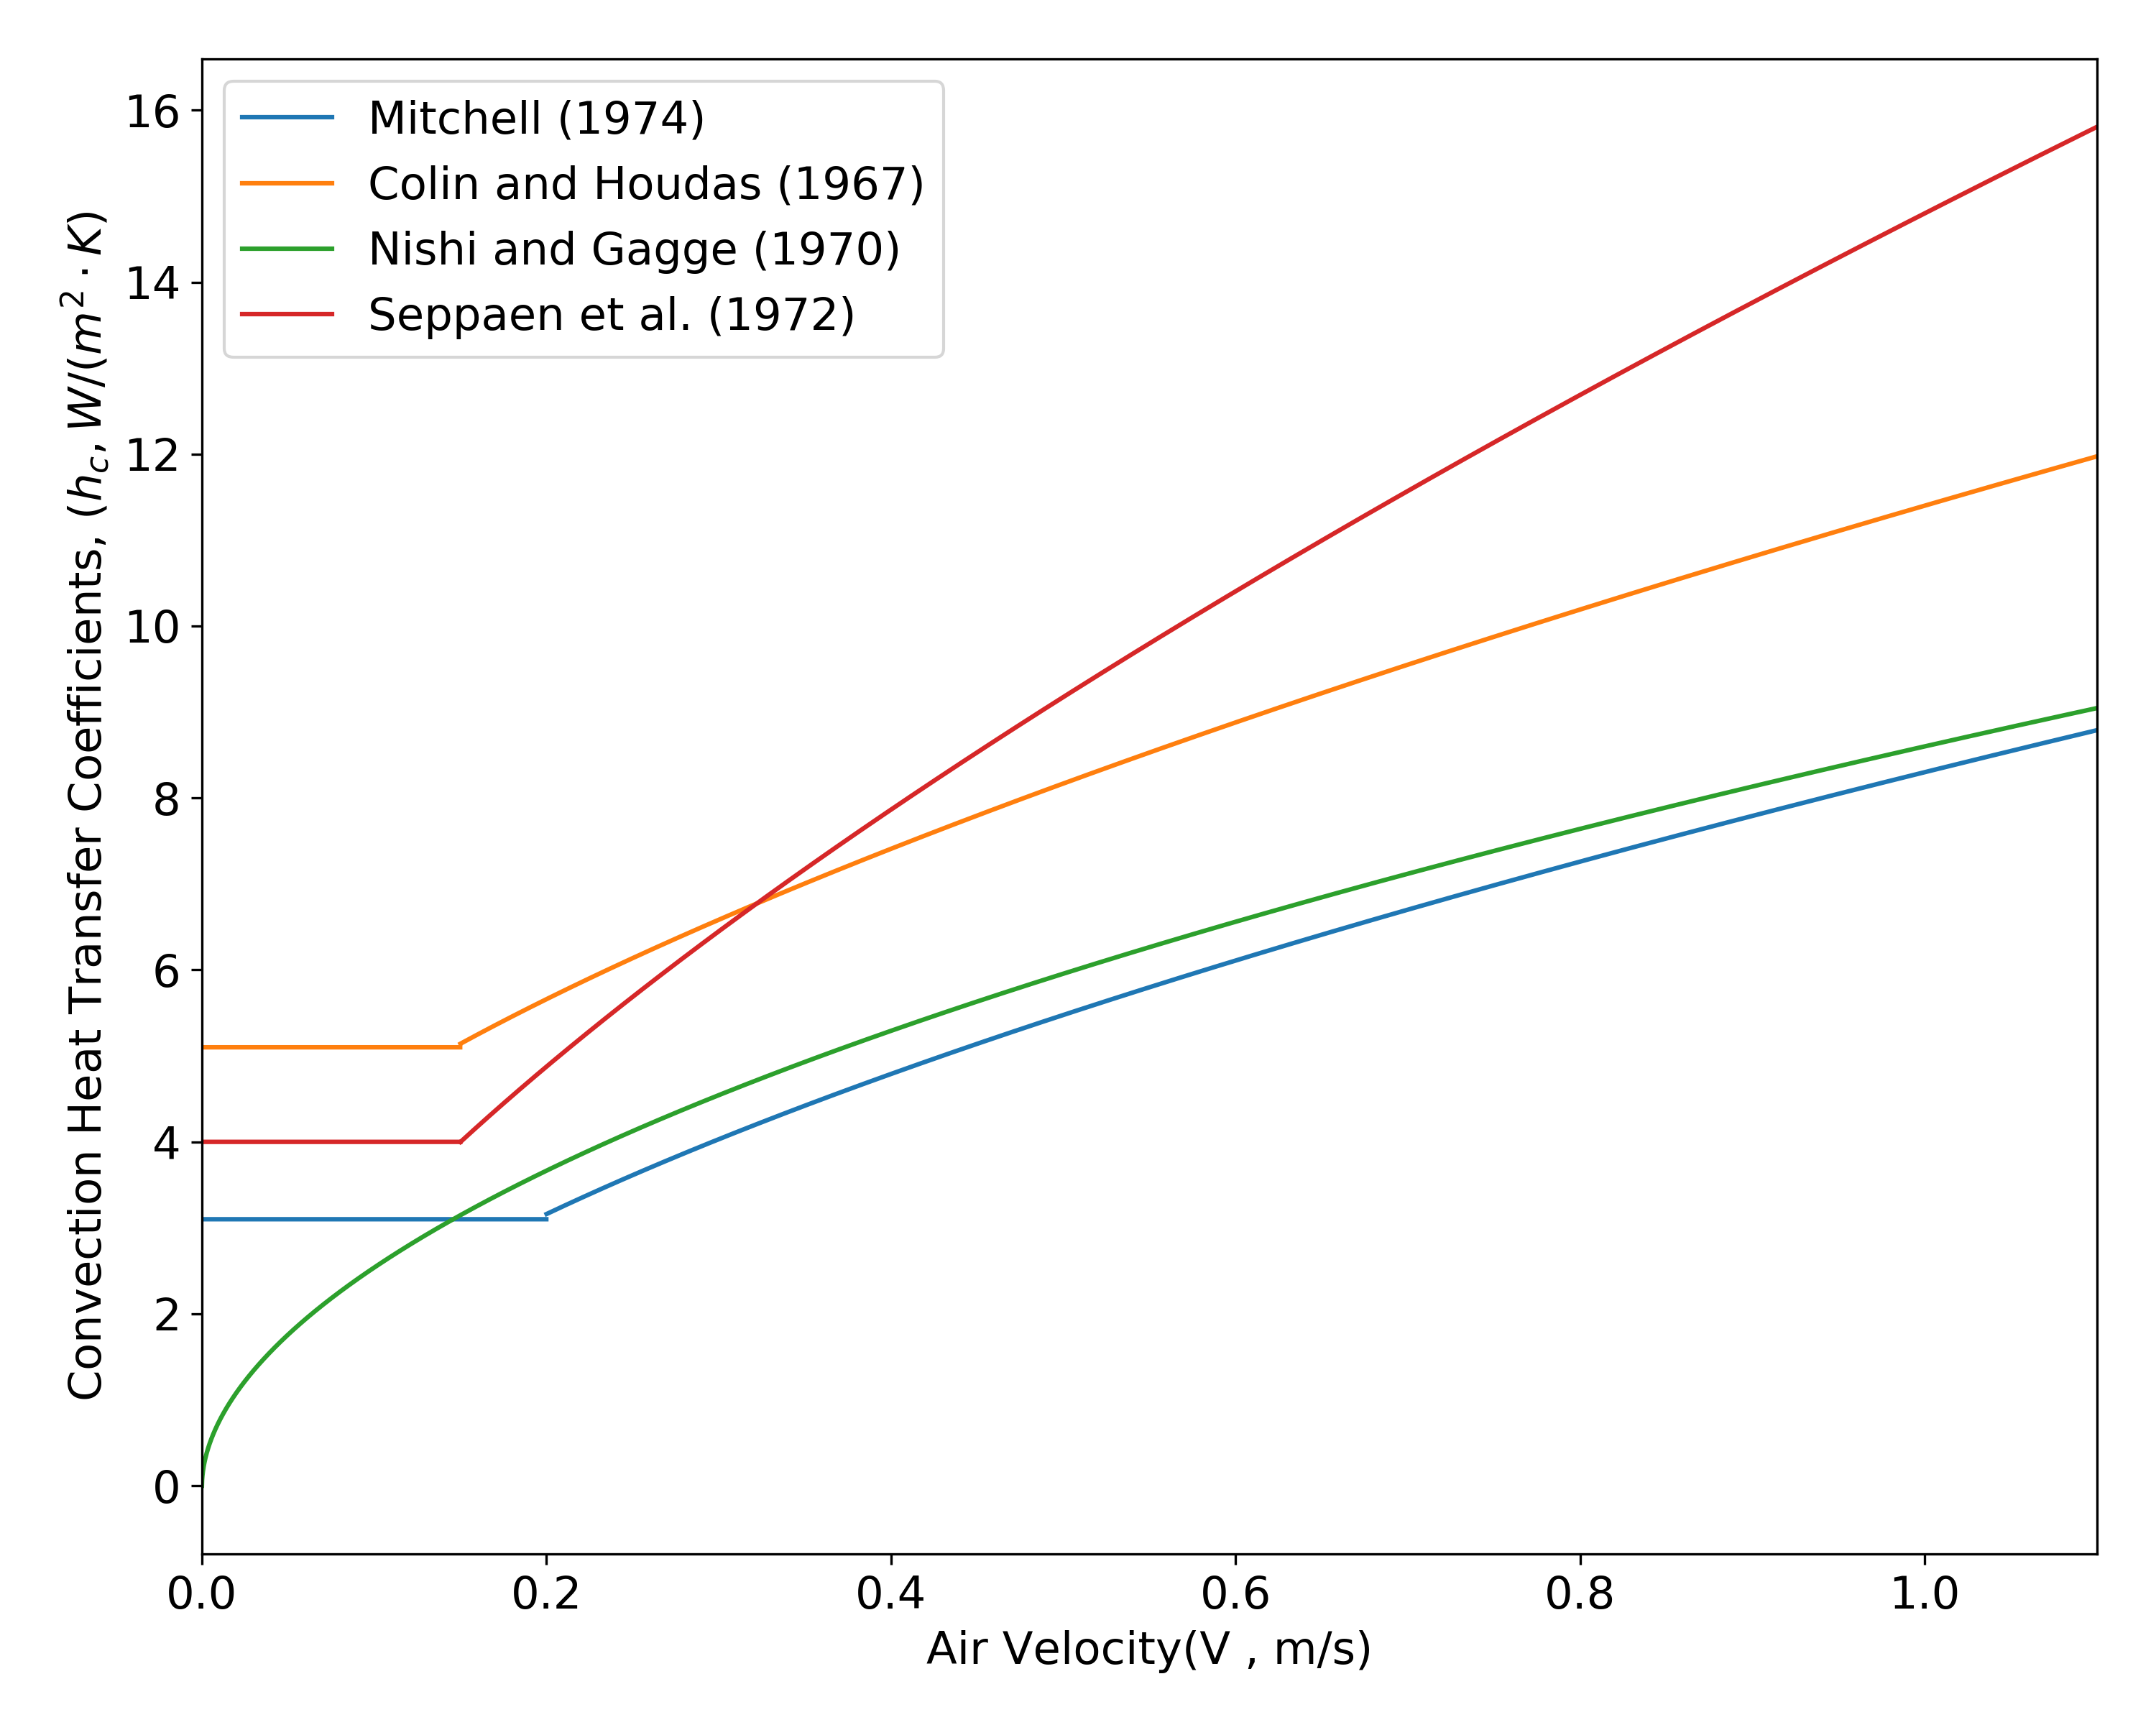
\includegraphics[width=0.5\textwidth]{figures/hcs4.png}
            \caption{$h_c$ with relation to air speed $V_a$ as defined in ASHRAE Handbook - Fundamentals 2009.}
            \label{fig:hc4s}
    \end{figure}
        %Operative temperature as the indicator of thermal comfort. Background and current range of applicable usages.
    Observing the relationship between the air velocity and resulting $h_c$, there is a very interesting relationship between the air velocity and the resulting operative temperature when substituting the expressions for $h_c$ in Table~\ref{tab:hcs} to Equation~\ref{eq:top}.
    \afterpage{\noindent
    \begin{figure}
            \centering
            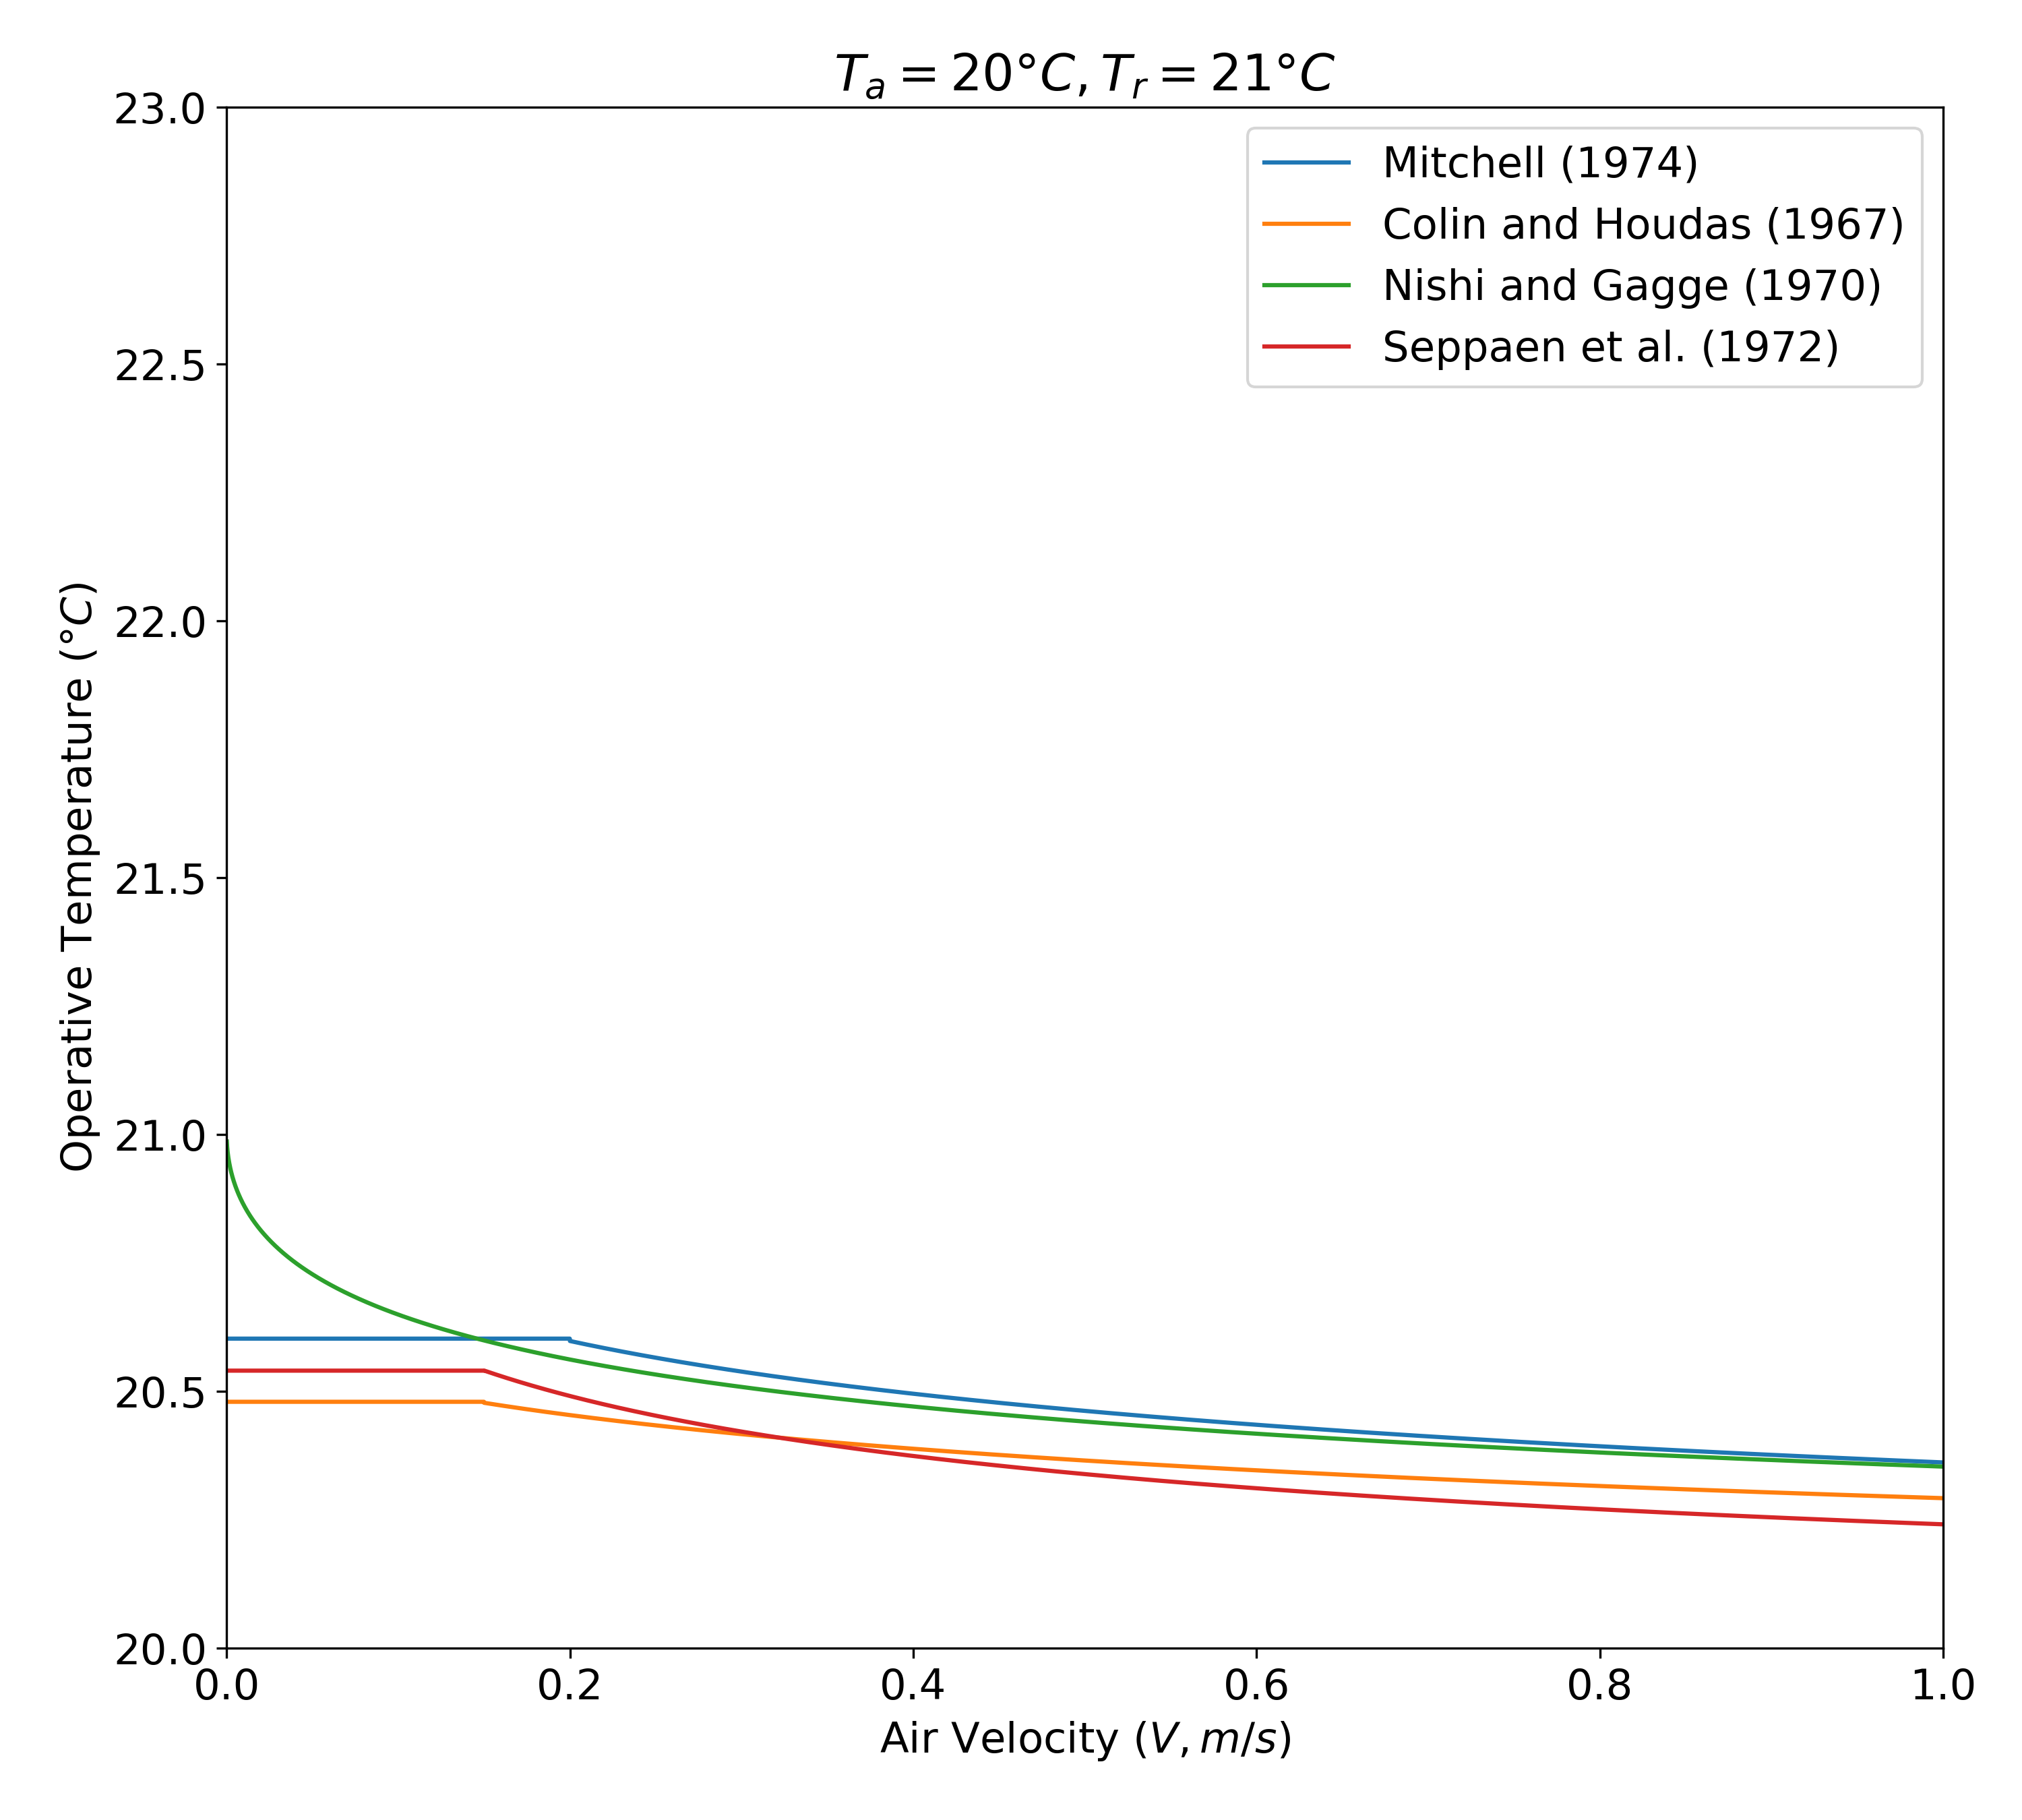
\includegraphics[width=0.49\textwidth]{figures/Ta20_Tr21.png}
            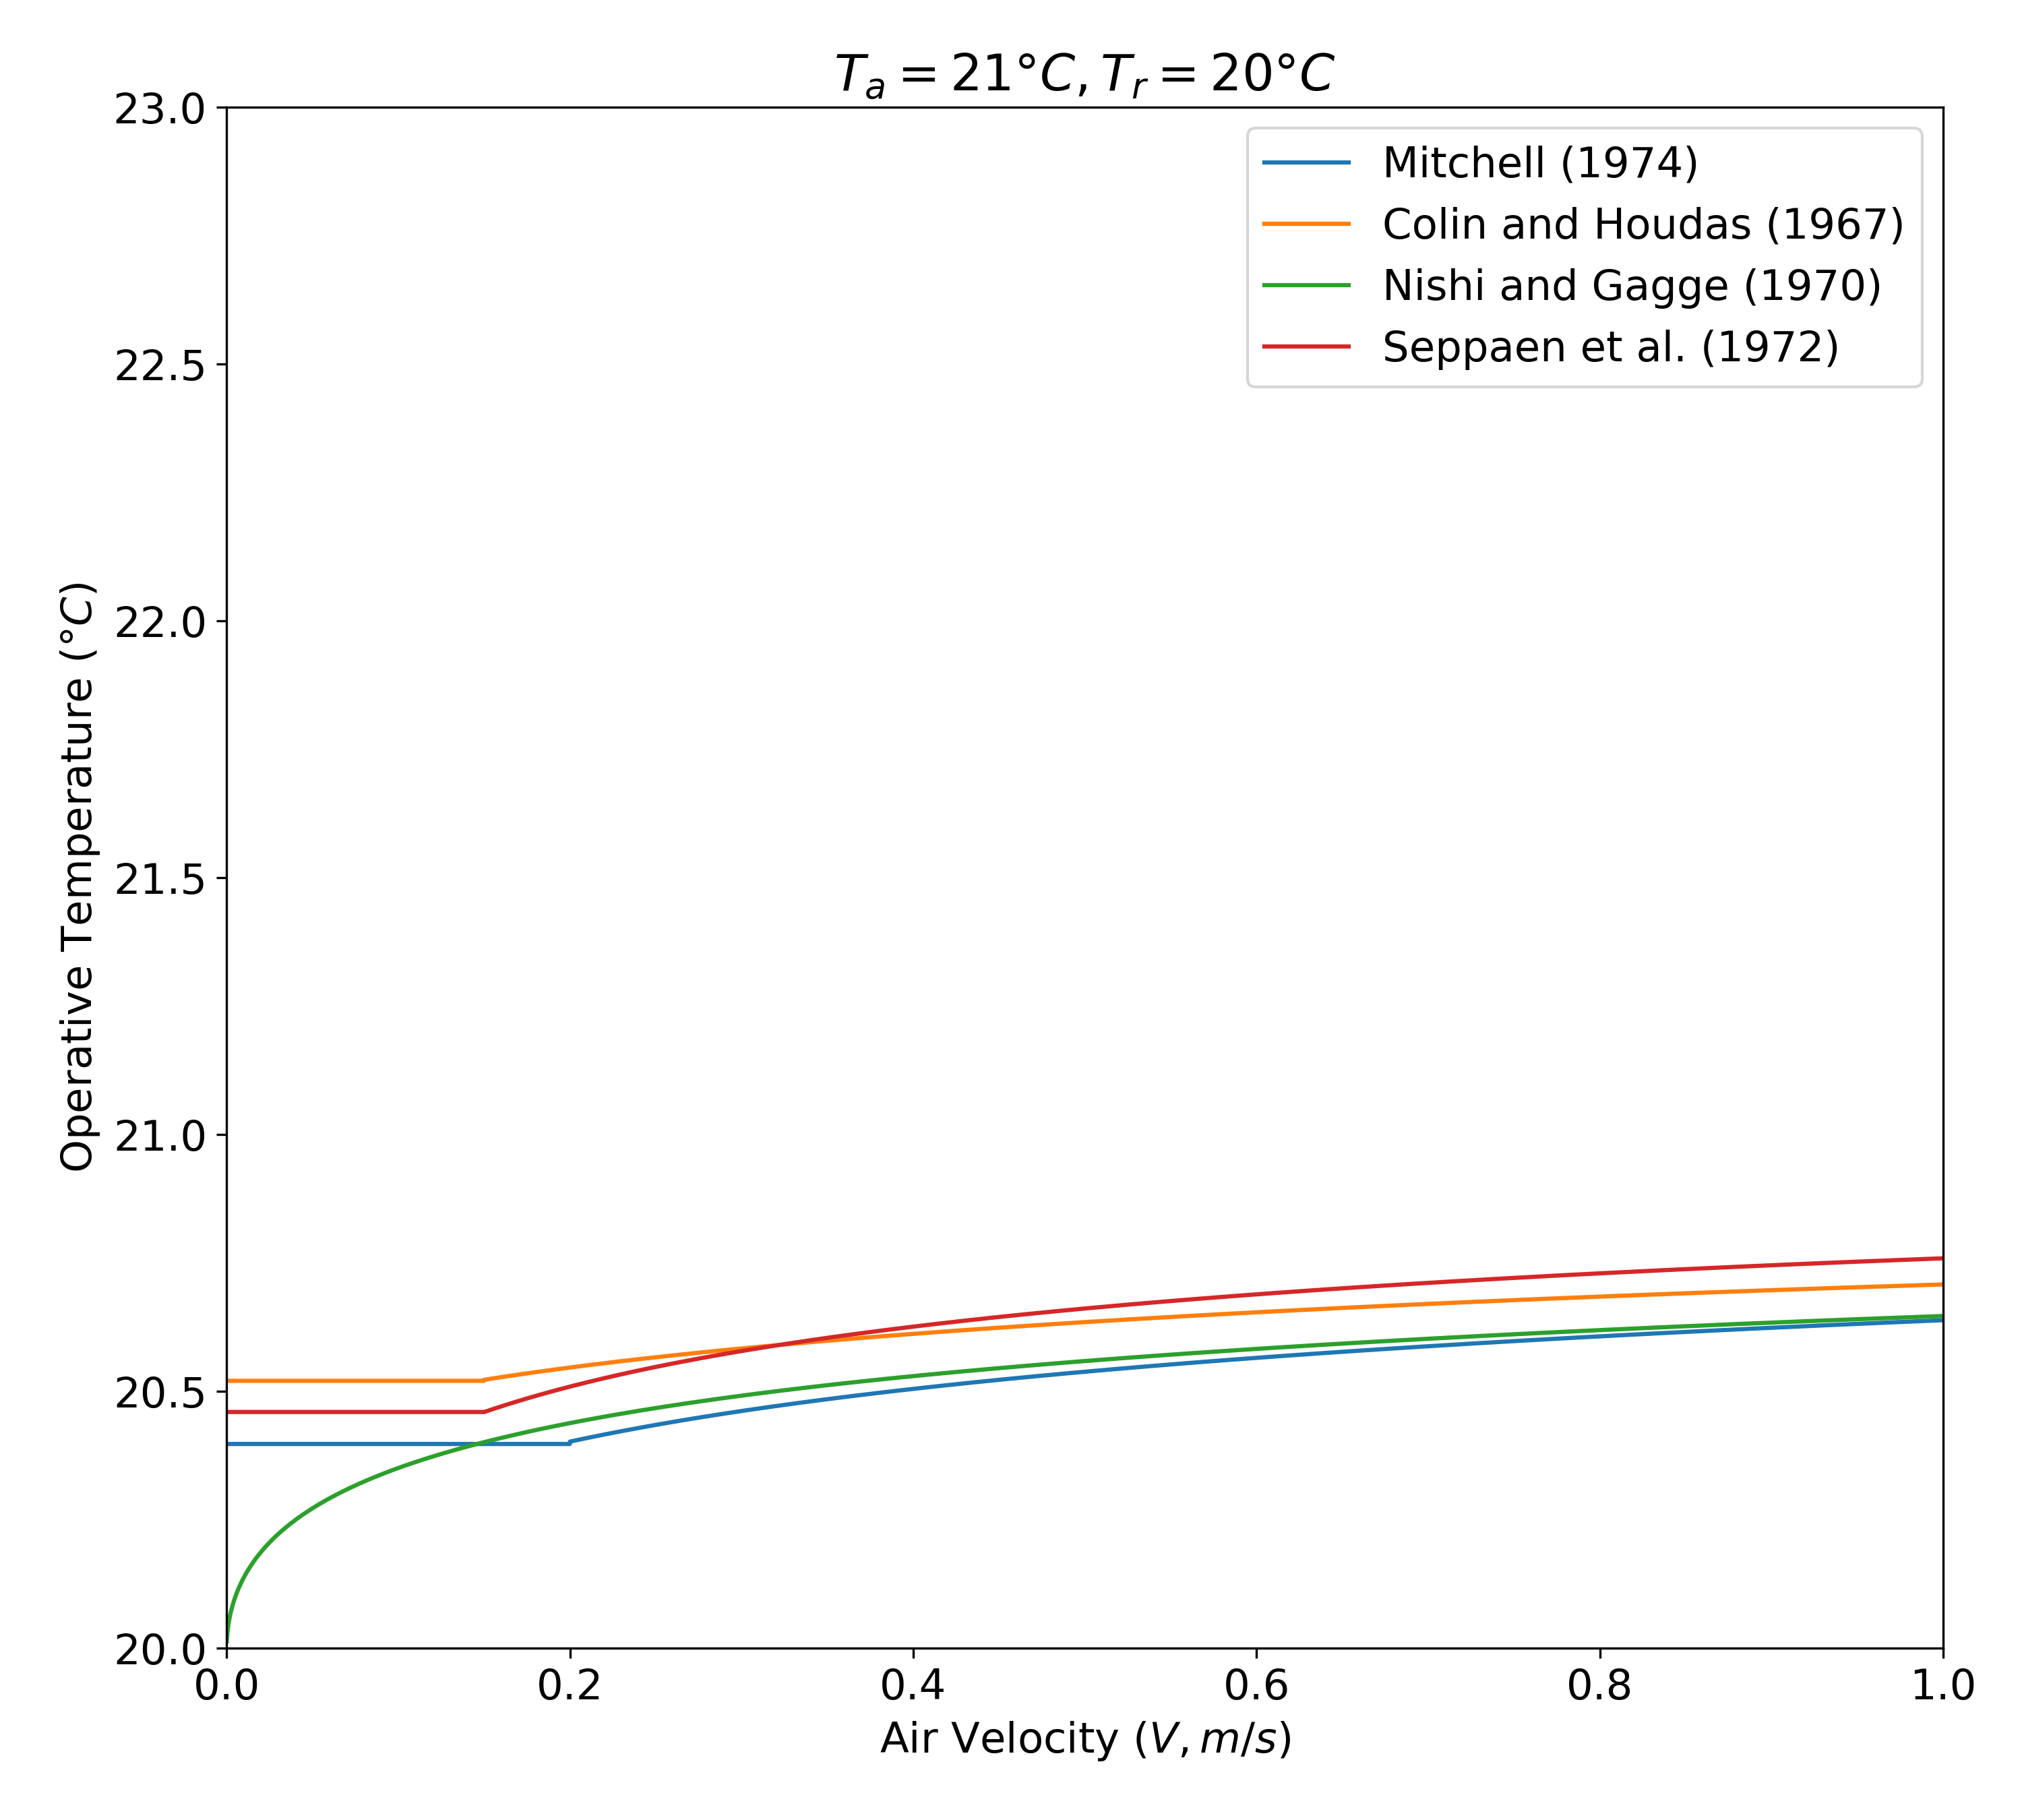
\includegraphics[width=0.49\textwidth]{figures/Ta21_Tr20.png}
            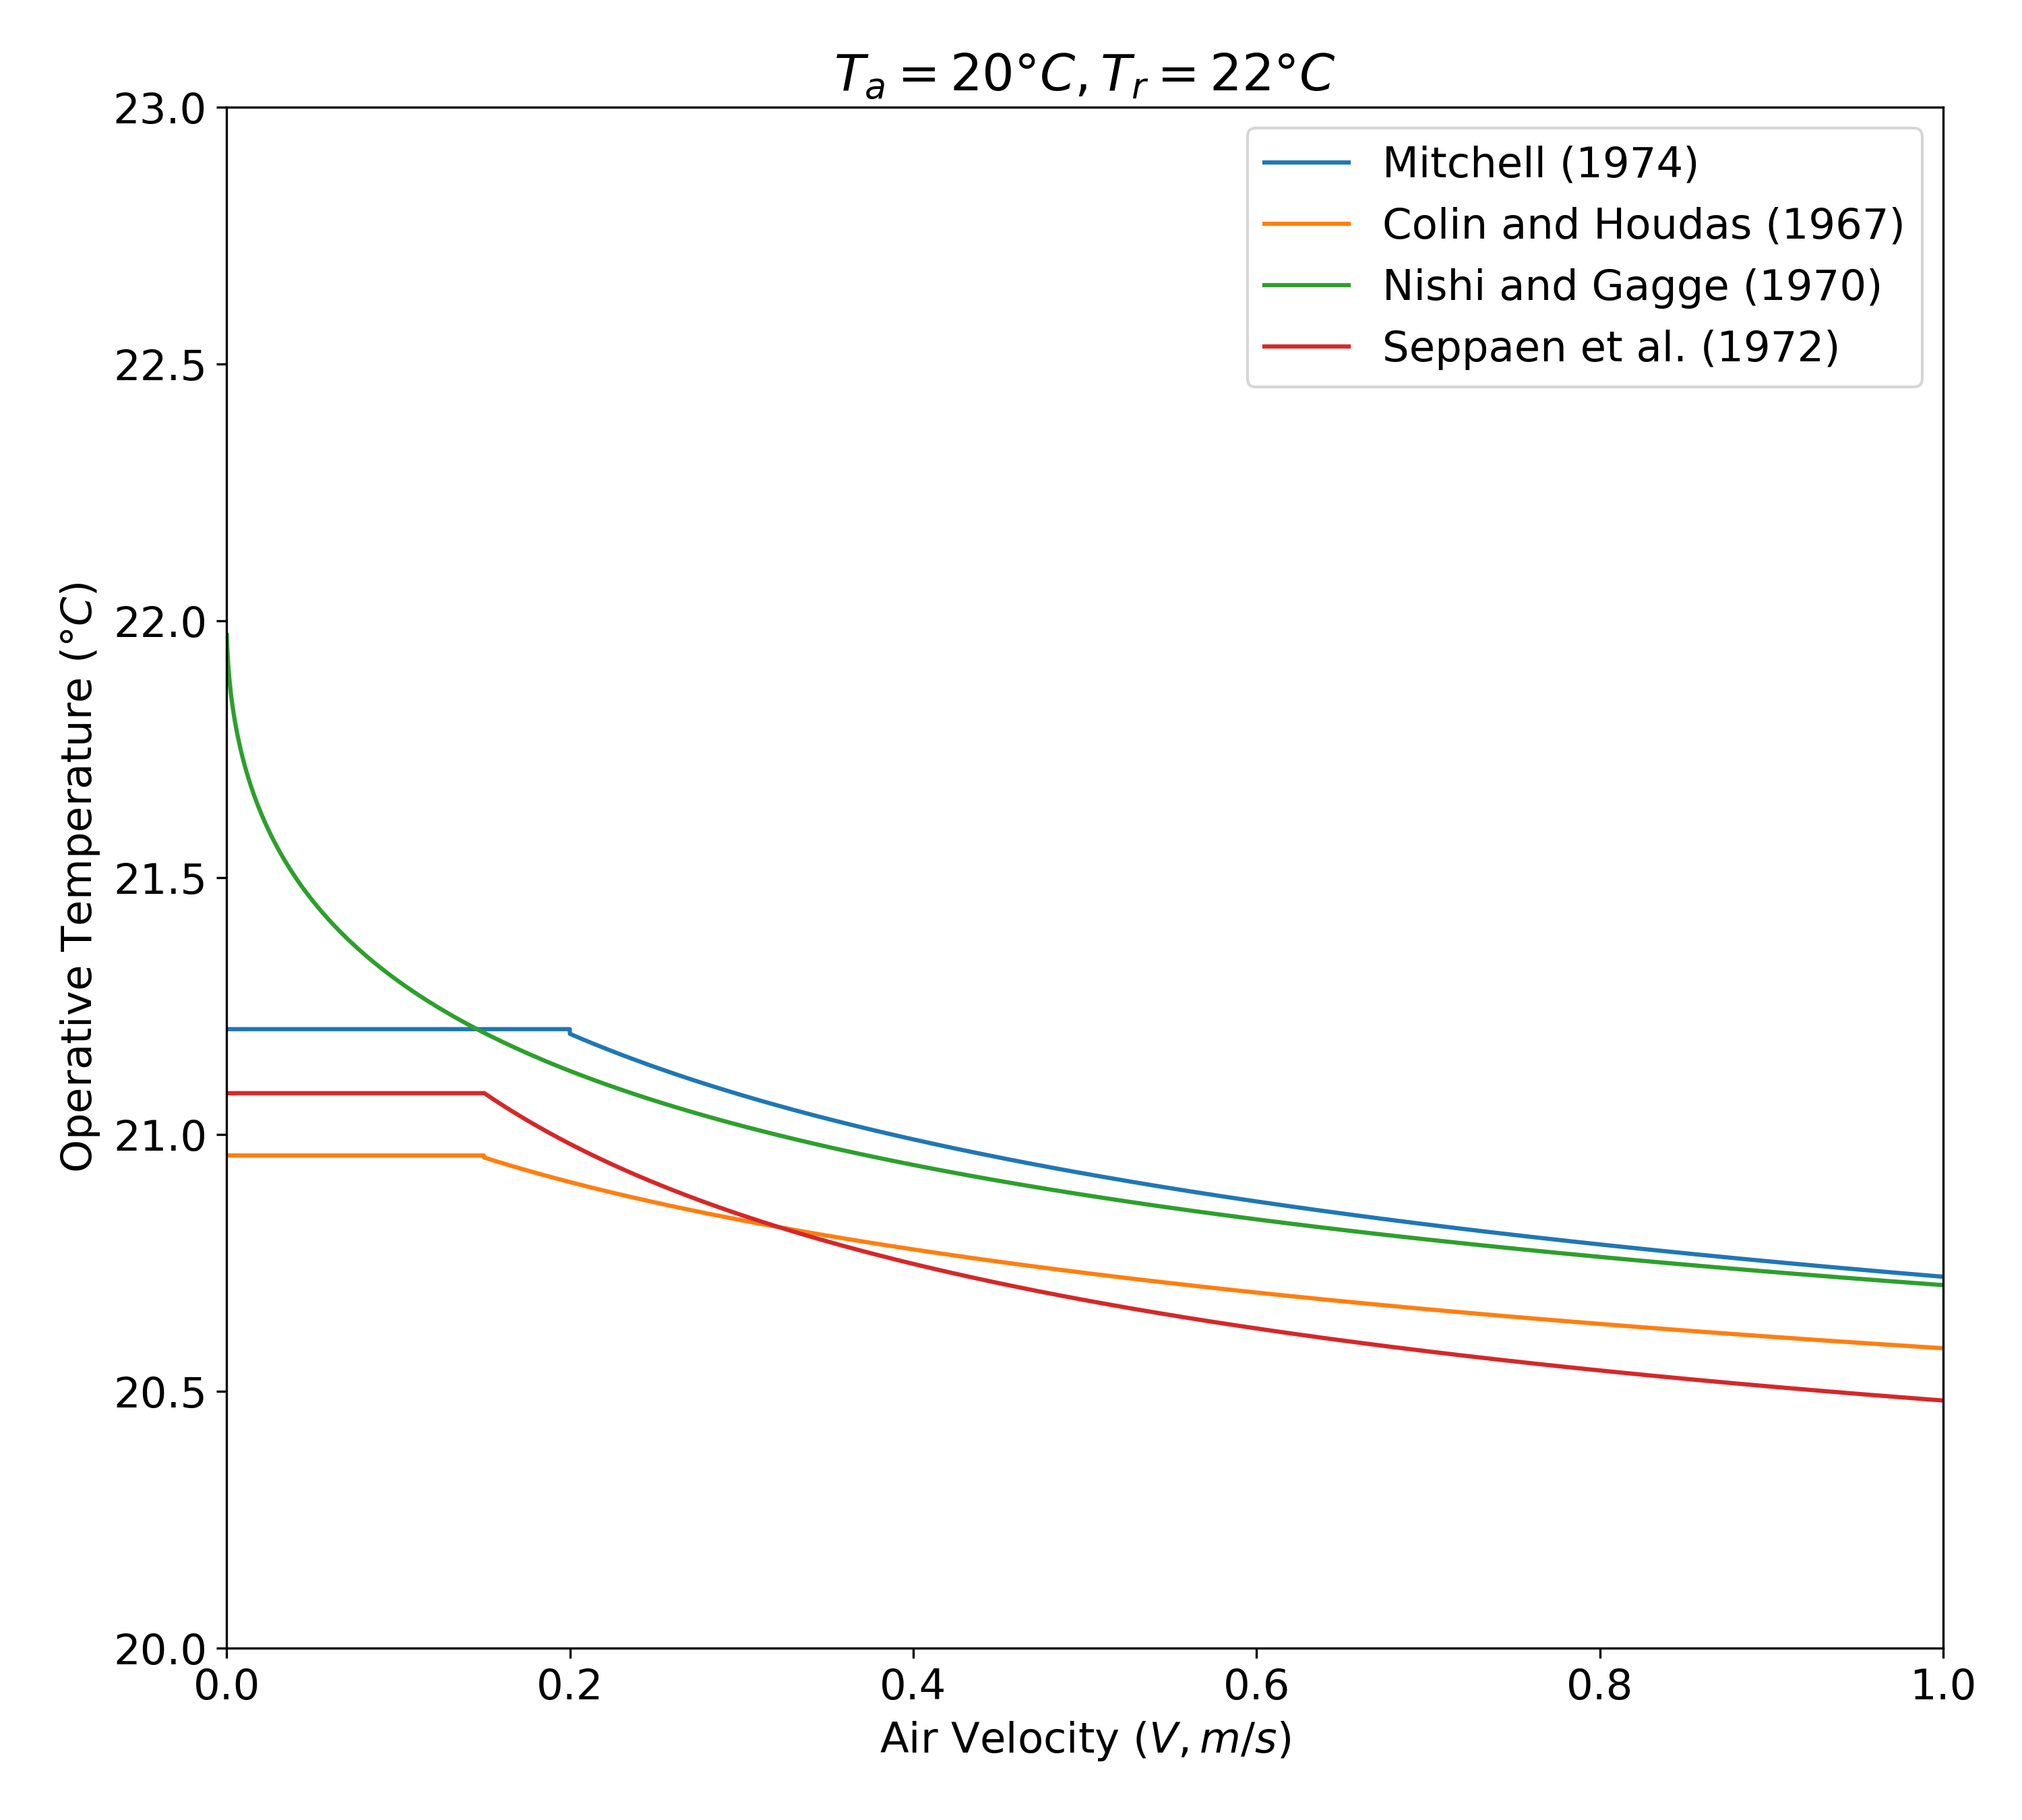
\includegraphics[width=0.49\textwidth]{figures/Ta20_Tr22.png}
            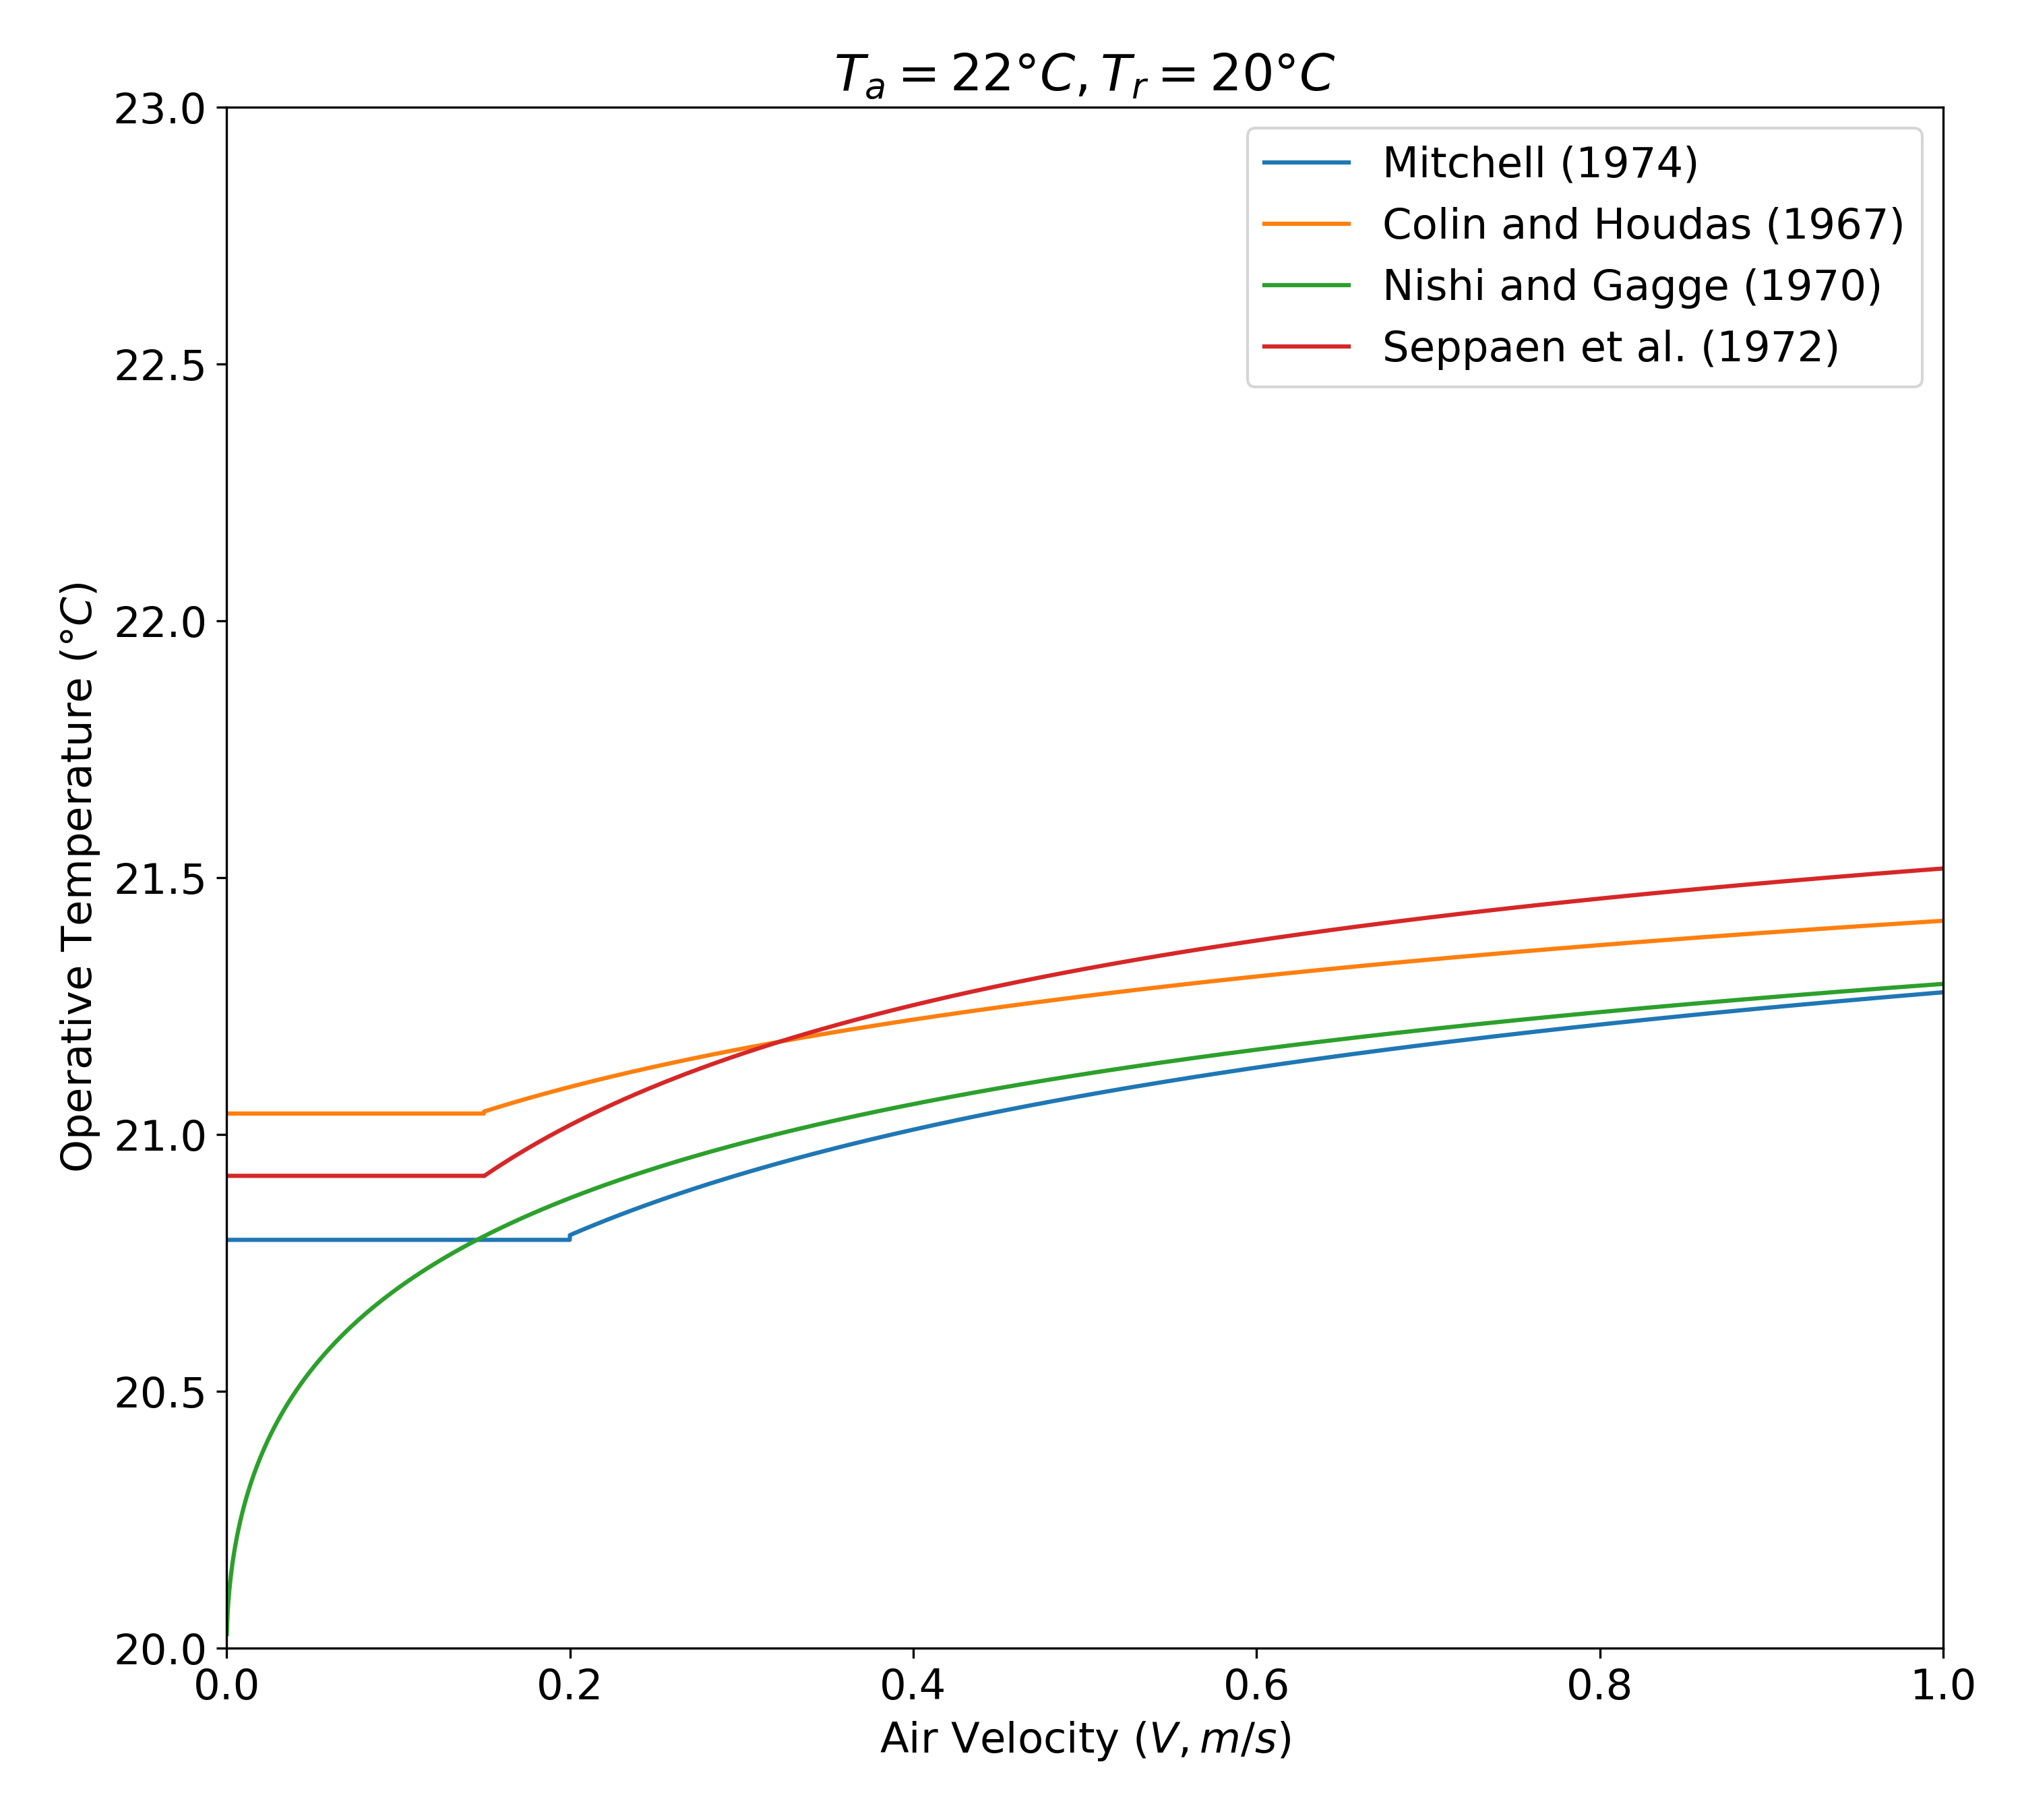
\includegraphics[width=0.49\textwidth]{figures/Ta22_Tr20.png}
            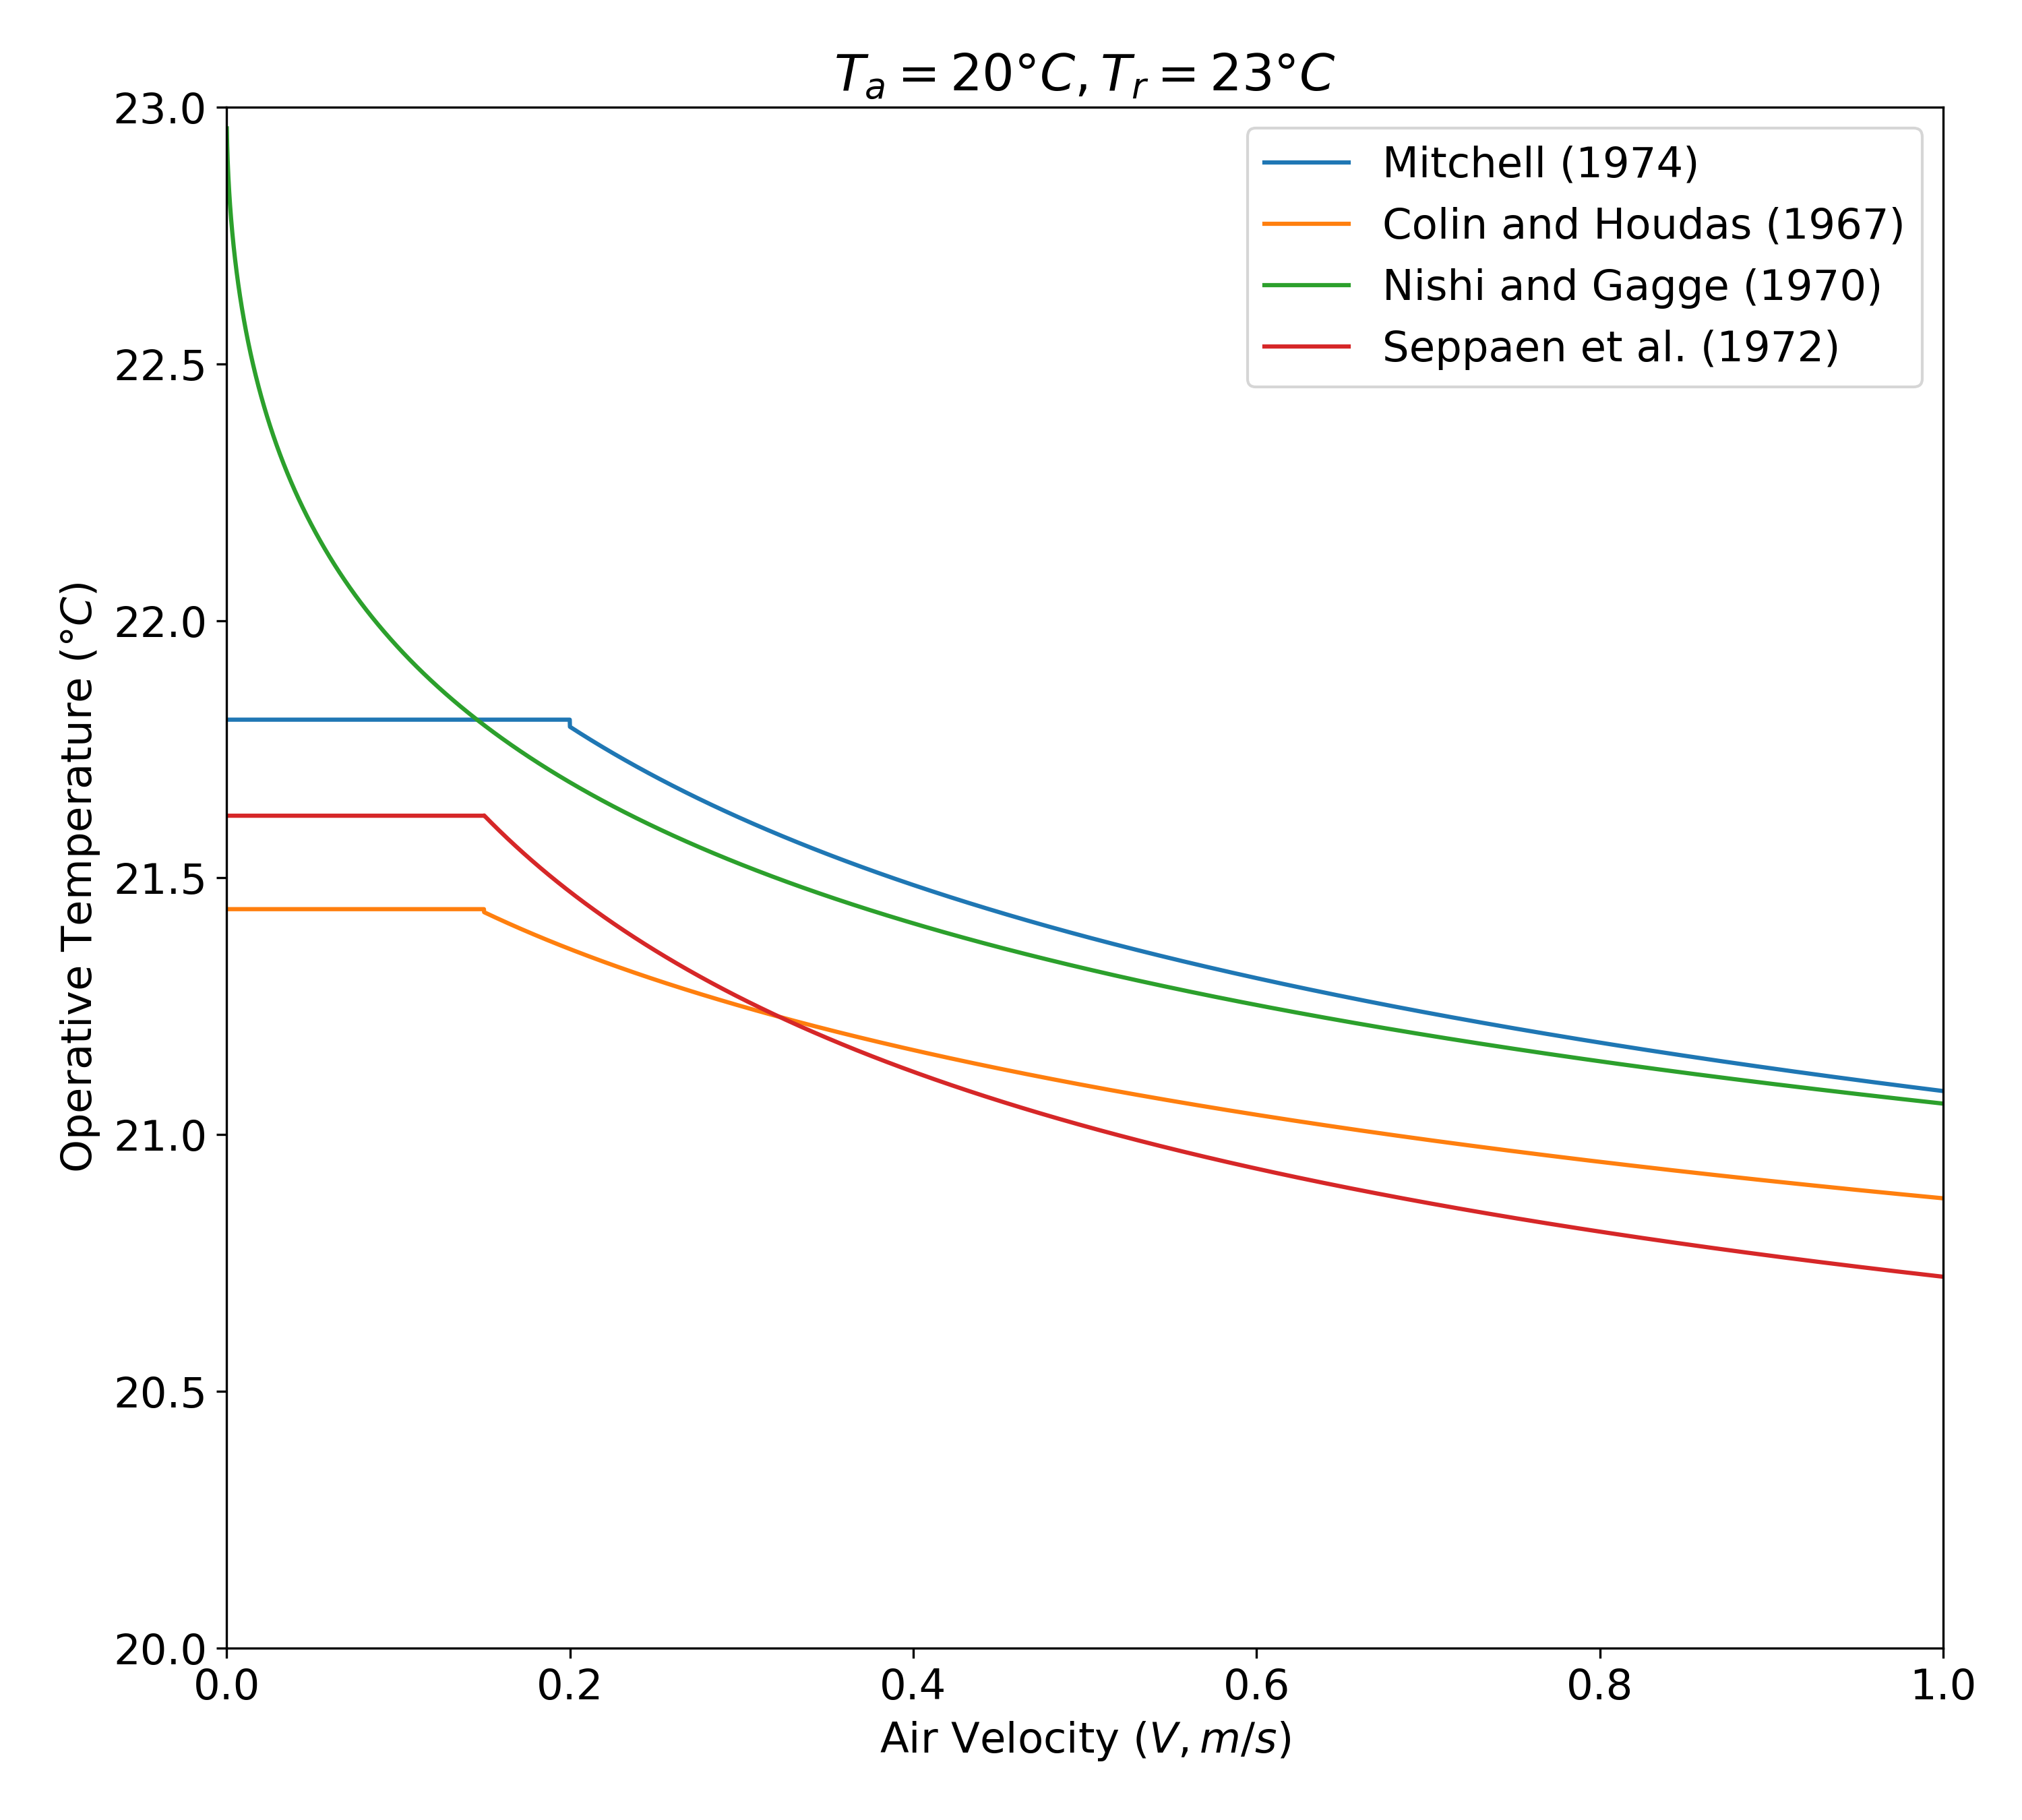
\includegraphics[width=0.49\textwidth]{figures/Ta20_Tr23.png}
            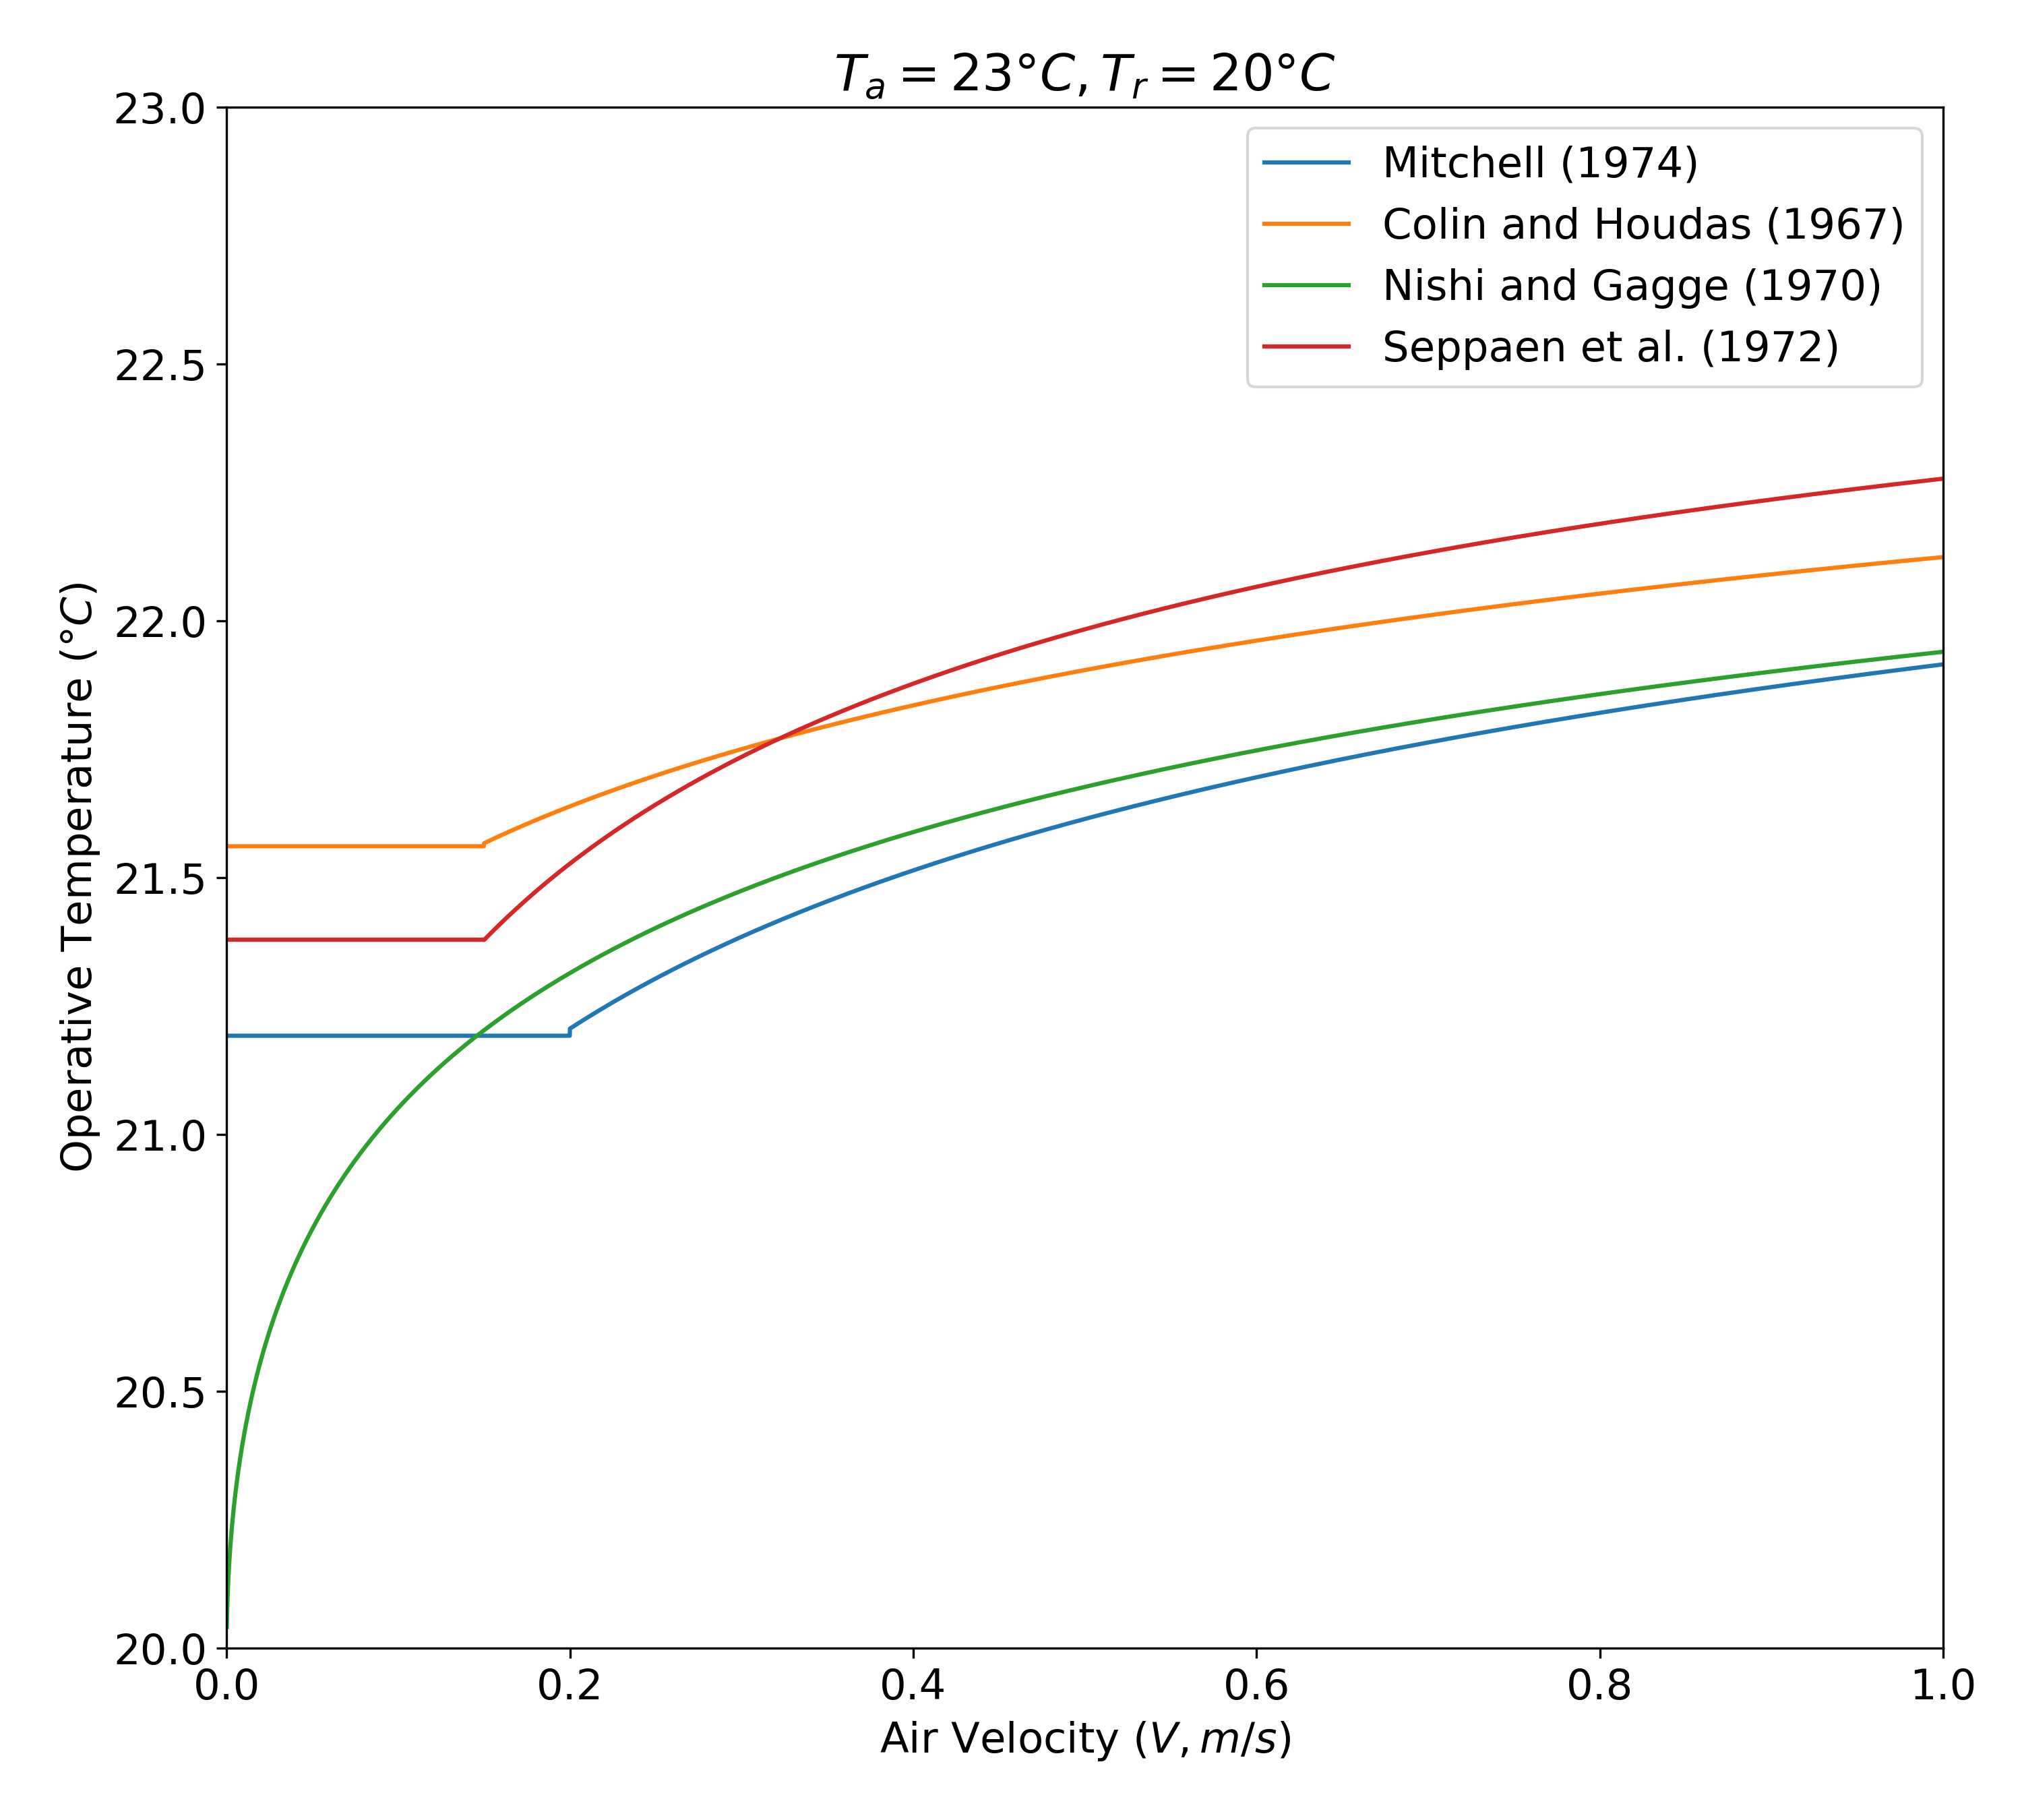
\includegraphics[width=0.49\textwidth]{figures/Ta23_Tr20.png}
            \caption{Relationship between air velocity ($V$) and operative temperature ($T_{op}$) when holding air temperature and mean radiant temperature constant.}
            \label{fig:Top_AR}
    \end{figure}
    }

    A very interesting phenomenon that we can observe, however, is the variation of operative temperature when holding air temperature and mean radiant temperature constant. As we're showing in Figure~\ref{fig:Top_AR}, increasing air velocity results in an increase of $T_{op}$ when $T_r$ < $T_a$, or a decrease of $T_{op}$ when $T_r$ > $T_a$.

    Alternatively, the definition of operative temperature as calculated per the formula given by ASHRAE 55-2017, where parameter $A$ is selected with respect to air velocity, or $V_a$. $A$ is evaluated at 0.5 when $V_a < 0.2m/s$, 0.6 when $V_a$ is between 0.2 and 0.6 $m/s$, and 0.7 when $V_a$ is between 0.6 and 1.0 $m/s$. As pointed out by SOMELIT, the overall clothing surface of a hypothetical average occupant is roughly 33.4 $\degree C$, thus any increase in $V_a$ when the ambient air temperature $T_a$ is below this number should be enhancing the convective heat transfer between the body and the surrounding environment, thus resulting in a decrease in perceived temperature. The operative temperature, in these cases, however, increases as the air velocity increases, which will result in the opposite direction of the prediction of thermal comfort. We believe this is a significant caveat of operative temperature to be used as a metric for thermal comfort assessment and would like to emphasize this in the current paper. More importantly, if we were to look back to the expression of operative temperature in Equation~\ref{eq:top}, it is evident that the definition itself is just a weighted average of air temperature and mean radiant temperature, which can easily become problematic when one of the heat transfer coefficient becomes much larger than the other - in this case $h_c > h_r$.

    Alternatively, the operative temperature can also be calculated from Equation~\ref{eq:opA55} to behave the same as indicated in Figure~\ref{fig:hc4s} where the operative temperature increases with increase of air velocity $V_a$ when $T_a > T_r$, which is the opposite of how an occupant exchanges heat with the surrounding environment as suggested by ASHRAE Standard 55-2017\cite{ansi/ashrae_standard_2017}. This will, again, not solve the effect of how higher $h_c$ influences
        \begin{equation}
            t_o = At_a + (1-A)\bar t_r\label{eq:opA55}
        \end{equation}

    Consequently, we believe there is a clear limitation of operative temperature to be used in indoor environment when radiant cooling is coupled with forced convection. Under scenarios created by such systems, the resulting operative temperature could be very misleading, i.e. increasing with the increase of air velocity despite the perceived temperature should have decreased for a hypothetical occupant. Examples that such a combination could exist are not uncommon:
    %DOAS + Chilled beam + forced convection? Open to examples!
\subsubsection{Predicted Mean Vote}
        Predicted Mean Vote (PMV) is a very popular concept in describing indoor thermal comfort. Developed in the 1970s, Fanger's  PMV model is based on both thermoregulation and heat balance theories as well as laboratory and climate chamber study results. The PMV model takes four physical variables (also referred to as environmental variables, i.e. $T_a$, $V_a$, MRT and relative humidity $\phi$) and personal variables (level of activity and clothing). Fanger's PMV model takes the six variables and produces a score that corresponds to the ASHRAE thermal sensation scale and represent the average thermal sensation felt by a large group of occupants \cite{ashrae_thermal_2003,fanger_thermal_1970}.

        There are some obvious benefits of using PMV. With the improvements in environmental control technologies, and the growth in personal wealth and office sizes (McIntyre, 1984), the need of better indoor environment requires a solution to predict the optimum temperature for a group of occupants, which can then be achieved by architects and engineers. Since its proposition in 1970, the PMV model has become the internationally accepted model for predicting and representing the mean thermal sensation vote by a large group of occupants for a set of given environmental variables. It has also since became the guideline for multiple international standards, where both ISO and ASHRAE indicated that a comfortable indoor environment can be insured when the PMV is kepted at 0 with a tolerace of $\pm0.5$.

        %Inidividual differences
        This does not mean there are not caveats in using PMV to describe the thermal sensation of offucpants. To begin with, there is an obvious difference in what Fanger's model can predict when compared to thermal comfort. As Fanger himself admitted, the usage of the heat balance models describes the balance between the thermoregulatory system and the environmental variables `even if comfort does not exist'. The neutral thermal sensation of an average person is not the same thing as thermal satisfaction, acceptability or preference. As Charles has pointed out in 1993, it is entirely possible for the occupants to vote on a neutral thermal sensation scale and to not feel comfortable.
        Neglecting the personal factors that reflects on their individual thermo-regulation and personal psychophysics is Natsume 1992, Havenith 2002

        %gender
        The PMV/PPD model also considers the inter-individual differences irrelevant from a series of experiments conducted in the 1960s. Fanger concluded from the results that the neutral temperature of a large group of occupants was independent of age, build, menstrual cycle, time of day, color and crowdedness of the room or gender, race as well as national geographic locations\cite{fanger_thermal_1970}. van Hoof pointed out that the original PMV model only accounts for the approximately 1,396 students who wear standardized clothes in a sedentary activity in Denmark, which does not reflect the larger and more diverse demographics of occupants in real buildings\cite{van_hoof_quantifying_2007}. Subsequent studies have since showed that there is a substantial gender differences where female occupants tend to feel significant cooler (Hill/Parsons 2002), and could be less satisfied with room temperatures while preferring higher room temperatures. Fanger made a similar observation earlier and concluded women are more sensitive to deviations than men\cite{fanger_assessment_1973}. To this observation, Parsons proceeded to conclude that during identical clothing and activity, the gender differences in thermal comfort responses for neutral and slightly warm conditions are smaller.

        %applicability
        The applicability of PMV has also became the subject of debate in some of the more recent publications. Despite some early validation of the PMV as a valid index when a meta-danalysis is performed, Humphreys and Nicol\cite{humphreys_validity_2002} found evidence of PMV bias often exceeding 0.25 scale units, and could reach as much as 1.0 - and the larger the deviation from neutral, the larger the bias. Their results suggested that PMV is only reliable between -0.5 and 0.5 unlike the range of validity stated by Fanger in his dissertation \cite{fanger_calculation_1967} and ISO (-2.0 and 2.0). More recently,  Cheong et al. found PMV only correctly predict thermal sensation correctly one out of three times\cite{cheong_local_2007}. This limitation of the PMV and PPD model is, however, not very well understood by practioners who are simply seeking a better metric and/or better adaptive model for conducting quick analysis of the thermal comfort requirements of an existing design. For practical purposes in existing projects, it is therefore highly desirable for practitioners to have a more accessible parameter to use for new and existing buildings, particularly when there are only limited information regarding the occupants and their schedules. %Setting pretext for adaptive thermal comfort

        %Thermal comfort zone
		%Regarding the thermal comfort zone - anlaytical tool?
		The latest standard published on determining the indoor occupants' thermal comfort is the ANSI/ASHRAE Standard 55-2017, which supersedes ANSI/ASHRAE Standard 55-2013, which is partially in agreement with ISO 7730, published as the ASRAE 55 Thermal Comfort Tool by the Center of Built Environment at Berkeley in 2017(Insert web citation).

		%What is comfort zone - it's verbal definition and graphical representation
		As briefly introduced previously, the comfort zone is defined as combinations of air temperature, mean radiant temperature $\bar t_r$  and humidity that are predicted to be an acceptable thermal environment at particular values of air speed, metabolic rate and clothing insulation $I_{cl}$(ASHRAE Standard 2017). It's also more commonly understood as two overlapping zones represented on psychrometric chart, where the air conditions are solved from a PMV of -0.5 to 0.5. This graphical approach assumes the rest of the environmental parameters (MRT, air velocity) and personal parameters (metabolic rate and clothing factors) as constants, and is the most widely accepted representation of the concept. There are actually two different ways of obtaining these boundary lines at PMV of -0.5 and 0.5. %Need to present it?

		%How we determine the comfort zone - three ways in ASHRAE.
		To determine the boundary of the comfort zone, both ISO 7730 and ASHRAE Standard 55 provide guidelines on how to do the actual calculation. There are currently three methods outlined in ASHRAE Standard 55, which applies to diffrent ranges of average air speed. With air speed lower than 0.2 m/s and a humidity ratio smaller than 0.012 kg$\cdot H_2O/kg$ dry air, the graphic comfort zone method should be used, where the operative temperature can be determined by linear interpolation the upper and lower operative temperature limit with a given clothing insulation. Alternatively, the comfort zone's boundaries can also be determined by using the Analytical Comfort Zone Method. This method can be applied to metabolic rate between 1.0 and 2.0, and clothing factor between 0 to 1.5 for all humidity ratios. This method incorporates the PMV calculation method used by ISO 7730.


        %Do we need to go so far for PPD? Probably unnecessary but it would hurt...
\subsubsection{The adaptive comfort model}
    The adaptive approach, first suggested by de Dear and Brager \cite{de_dear_developing_1998} was developed to account for the occupant adaptibility in environments that have wider bandwith than air-conditionined buildings such as naturally ventilated buildings. According to de Dear and Brager, the PMV model is not applicable for these environments because it only partly accounts for the adaptation process and were results from limited laboratory studies. They therefore proposed an adaptive thermal comfort model for free-runnign buildings, linking the neutral temperature indoors to the outdoor monthly average temperatures. According to van Hoof, Fanger responded to this model in 2004 by pointing out that adaptation should be `a process of machines adapting to human requirements and ergonomics, not the adaptation of humans to technology'\cite{van_hoof_forty_2008}, but this did not stop the expansion of the usage of the adaptive thermal comfort model in the subsequent studies. The adaptive thermal comfort is currently included in the ASHRAE Standard 55 as an optional method that can be applied to naturally ventilated office buildings when outdoor temperature is between 10 and 33 $\degree C$. %Consider adding in the equations for this - but only after adding in the equations for PMV also

    %How wide is this currently?
	As suggested by ASHARE Standard 55, the adaptive model applies to indoor environments with air speeds beyond 0.3 m/s, specifically where occupants have better control over their own built environment. Although not explicitly addressing the occupants in the room, this model appears to have worked well for scenarios including open offices, classrooms, and many other cases of natural or hybrid ventilation. 
    
    %What is the adaptive thermal comfort?
	However, it is important to point out that a majority of the laboratory studies that appeared to have demonstrated the usage of the adaptive thermal comfort models are more commonly found in studies conducted in classrooms among younger children - who exhibits not only higher metabolic rates, higher activity levels and smaller muscle/fat ratio. It is important to point out that these studies are more conclusive may not be a coicidence, i.e. that the younger occupants of an indoor environment. However, as these experiments are, in fact, conclusive, understanding their results are far more important than what was previously observed. %Younger,students, open plan offices

    %Some of its limitations?
    Despite some clear strength over the PMV/PPD models, the first limitation of the adaptive thermal comfort its exclusion of the six input parameters of PMV that regards the human heat balance as as crucial component to consider for the indoor environment.

    Comparing to the oeprative temperature and the predicted mean vote, the adaptive thermal comfort model is much less specific, since it is a non-deterministic metric. The exploration of this model is a branch that stems out from
    %It comes out from Fanger's acceptance that there is a range of environmental conditions that people are 'in general comfortable', while Fanger's own model points to a deterministic range of comfort.

    The adaptive thermal comfort model also has an equivalent definition of the `comfort zone' for naturally ventilated spaces\cite{ashrae_ansi/ashrae_2013}. As outlined in the ASHRAE Standard 55, the upper and lower 80\% accetability limit of the operative operative temperature can be calculated from its linear relationship with the prevailing daily outdoor air temperature. 
    %Also needs to refer to the human body exergy model, how it should be a range of exergy consumption rates that applies to the entire setup - or the lack thereof. We need to emphasize how important this is, and how we might be able to develop anything out of it. Specifically addressing these could require a single paragraph of the exergy consumption rate (alternative models?)
